\section{(Model-based) Goal-based Agents}\label{AI: Agent Programs/(Model-based) Goal-based Agents}


\begin{figure}[H]
    \centering
    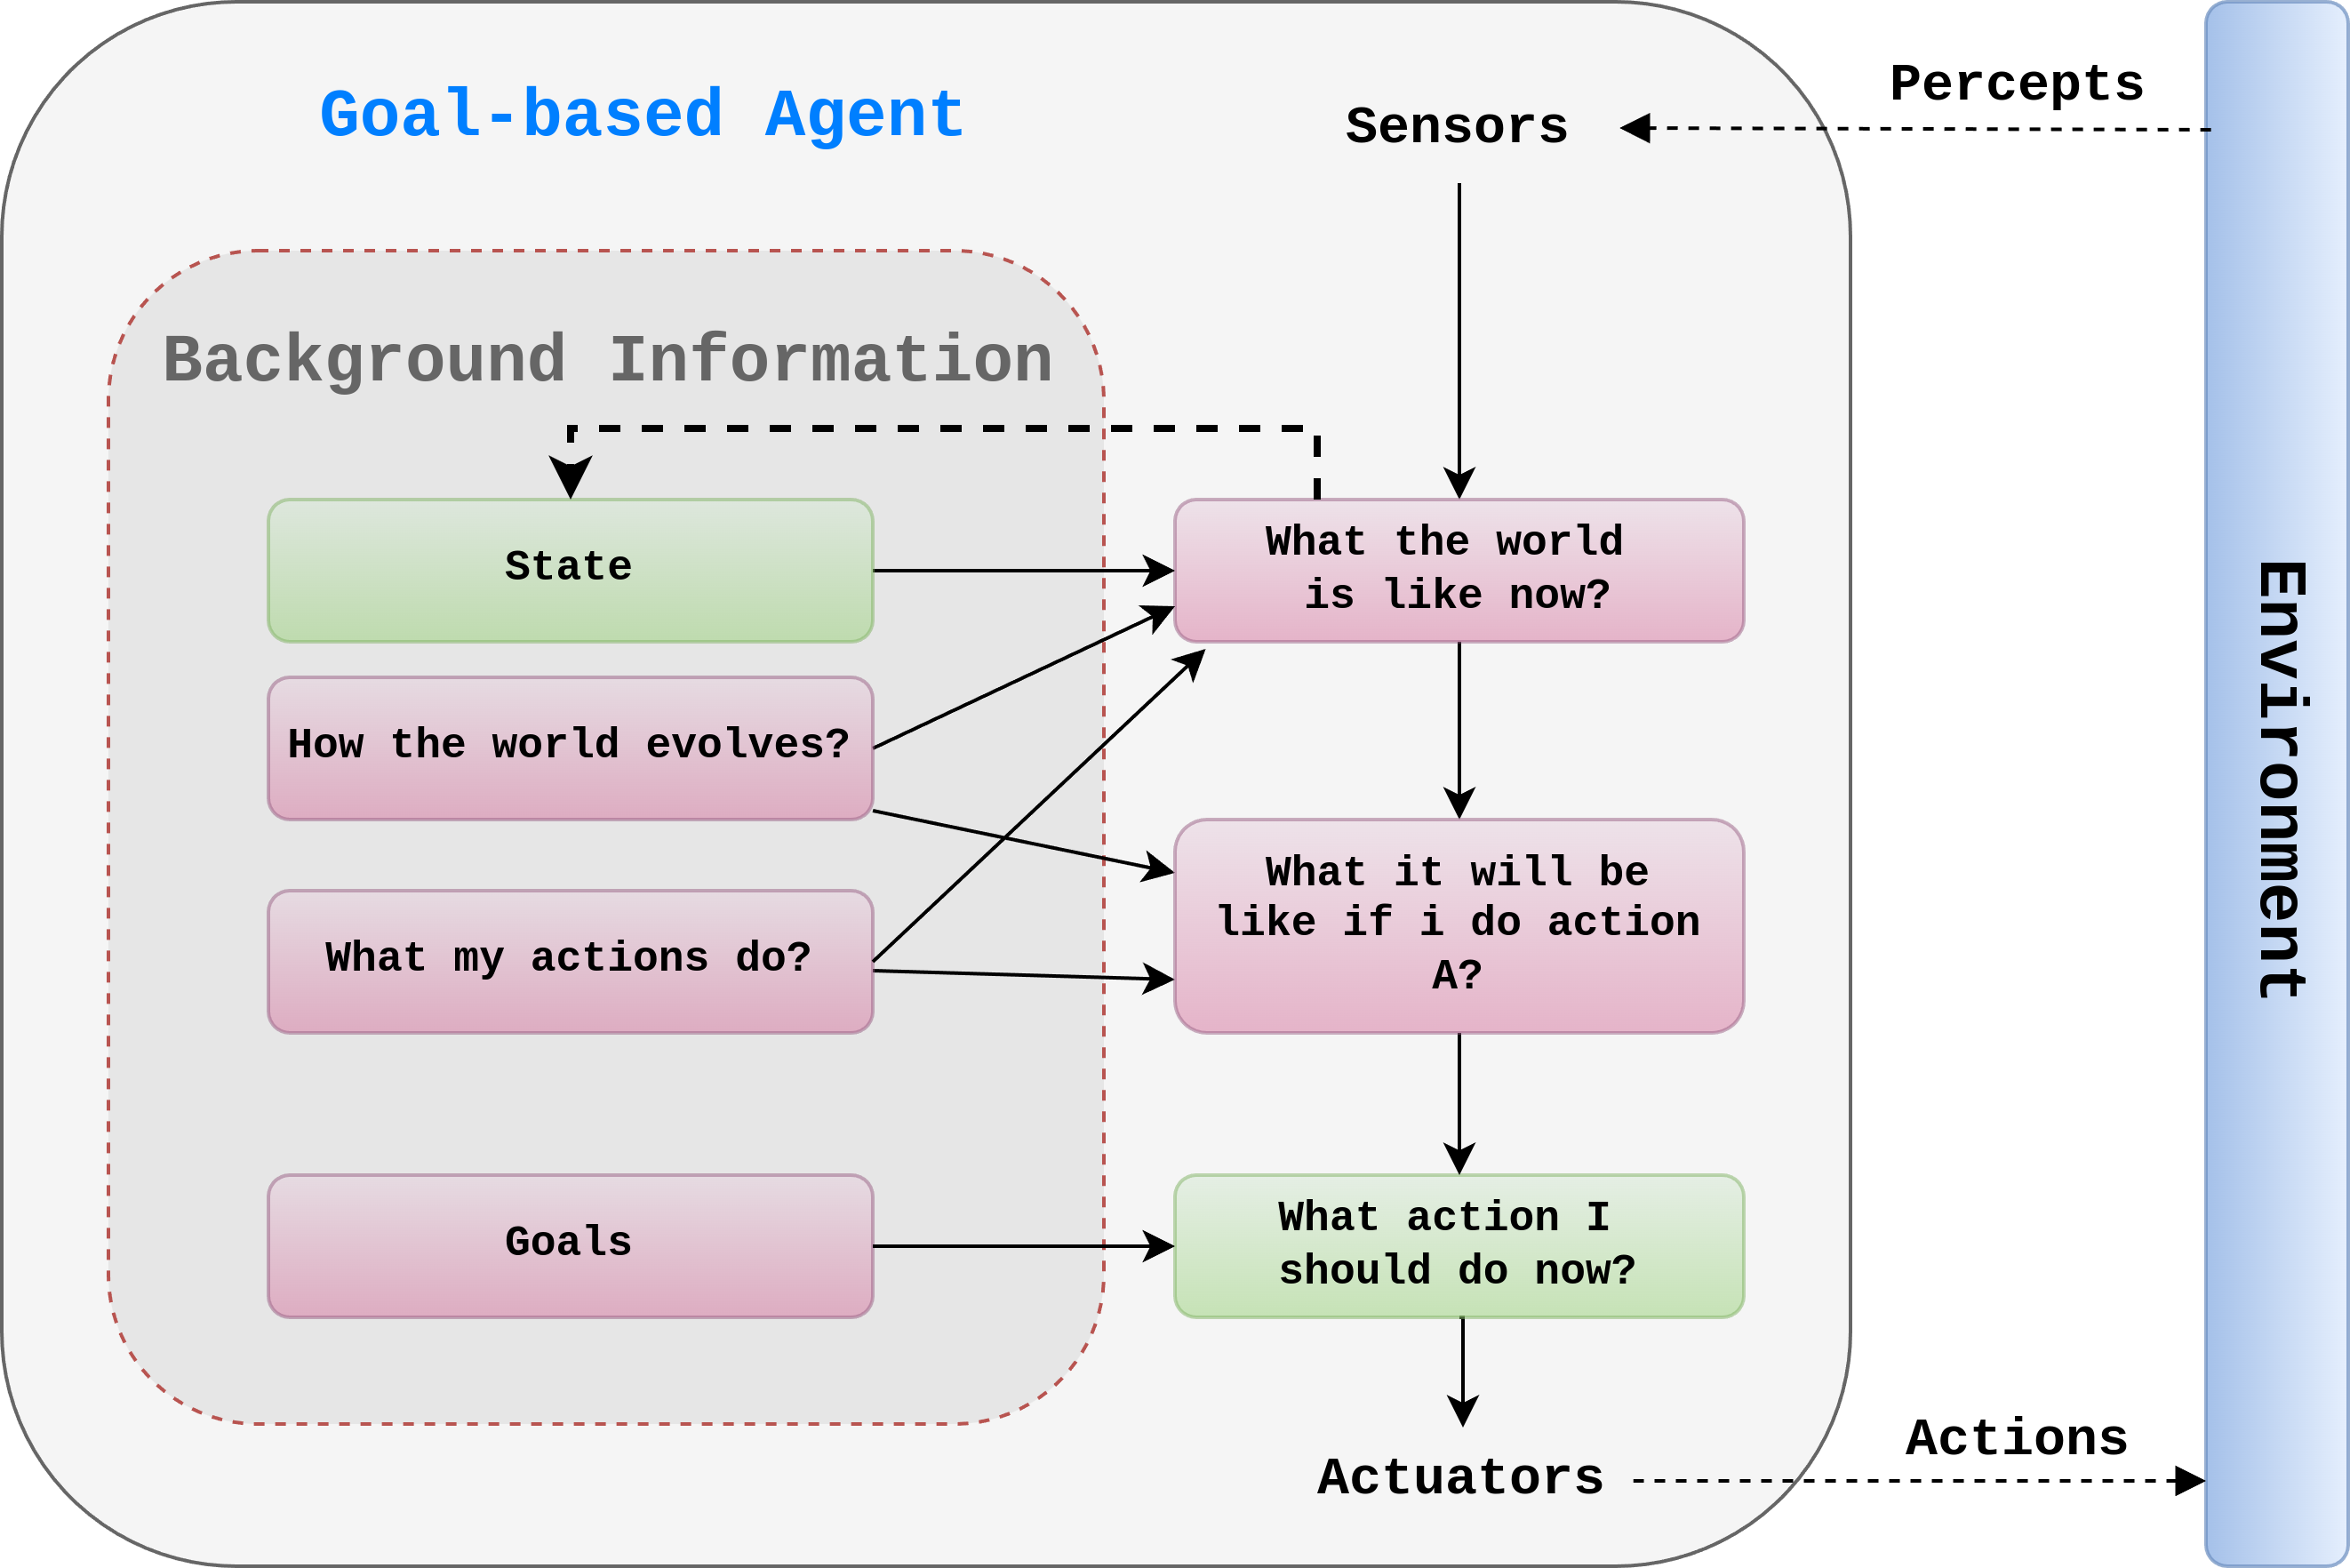
\includegraphics[
        width=0.5\linewidth, 
        height=6cm, 
        keepaspectratio
    ]{images/artificial-intelligence/ai-agents/agents-Goal-based-agent.png}
    \caption*{A model-based, goal-based agent. \cite{common/online/tools/draw.io}}
\end{figure}



\begin{enumerate}[itemsep=0.2cm]
    \item As well as a current state description, the agent needs some sort of \textbf{goal} information that describes situations that are desirable.
    \hfill \cite{ai/book/Artificial-Intelligence-A-Modern-Approach/Russell-Norvig}

    \item  The agent program can combine this with the model (the same information as was used in the modelbased reflex agent) to choose actions that achieve the goal.
    \hfill \cite{ai/book/Artificial-Intelligence-A-Modern-Approach/Russell-Norvig}

    \item Sometimes goal-based action selection is straightforward - for example, when goal satisfaction results immediately from a single action. Sometimes it will be more tricky - for example, when the agent has to consider long sequences of twists and turns in order to find a way to achieve the goal.
    \hfill \cite{ai/book/Artificial-Intelligence-A-Modern-Approach/Russell-Norvig}

    \item decision making of this kind is fundamentally different from the condition–action rules \\
    decision making involves consideration of the future - both \textit{“What will happen if I do such-and-such?”} and \textit{“Will that make me happy?”}.
    \hfill \cite{ai/book/Artificial-Intelligence-A-Modern-Approach/Russell-Norvig}

    \item It is \textbf{not reflexive}. It takes calculated decisions.

    \item Although the goal-based agent appears less efficient, it is more flexible because the knowledge that supports its decisions is represented explicitly and can be modified.
    \hfill \cite{ai/book/Artificial-Intelligence-A-Modern-Approach/Russell-Norvig}

    \item Goals just provide a crude binary distinction between “happy” and “unhappy” states.
    \hfill \cite{ai/book/Artificial-Intelligence-A-Modern-Approach/Russell-Norvig}

    \item SEE: subfields of AI devoted to finding action sequences that achieve the agent’s goals: (TODO)
    \begin{enumerate}
        \item Search
        \item Planning
    \end{enumerate}
\end{enumerate}

